%%% Preamble
\documentclass[paper=a4, fontsize=11pt]{report}
\usepackage[utf8]{inputenc}
\usepackage[T1]{fontenc}
\usepackage{fourier}
\usepackage[french]{babel}
\usepackage[protrusion=true,expansion=true]{microtype}	
\usepackage{amsmath,amsfonts,amsthm} % Math packages
\usepackage[pdftex]{graphicx}	
\usepackage{url}
\usepackage{pdfpages}
\usepackage{todonotes}
\usepackage[a4paper, body={17cm,26cm}]{geometry}
\usepackage{float}
\usepackage{framed}
\usepackage[toc,page]{appendix} 
\usepackage{multicol}


%%% Custom sectioning
\usepackage{sectsty}
\allsectionsfont{  \normalfont\scshape}
%\allsectionsfont{\centering \normalfont\scshape}

%%% Custom headers/footers (fancyhdr package)
\usepackage{fancyhdr}
\pagestyle{fancyplain}
\fancyhead{}											% No page header
\fancyfoot[L]{}											% Empty 
\fancyfoot[C]{}											% Empty
\fancyfoot[R]{\thepage}									% Pagenumbering
\renewcommand{\headrulewidth}{0pt}			% Remove header underlines
\renewcommand{\footrulewidth}{0pt}				% Remove footer underlines
\setlength{\headheight}{13.6pt}


%%% Equation and float numbering
\numberwithin{equation}{section}		% Equationnumbering: section.eq#
\numberwithin{figure}{section}			% Figurenumbering: section.fig#
\numberwithin{table}{section}				% Tablenumbering: section.tab#


%%% Define new commands
\newcommand{\horrule}[1]{\rule{\linewidth}{#1}} 	% Horizontal rule
\renewcommand{\bf}[1]{\textbf{#1}}
\renewcommand{\it}[1]{\textit{#1}}

\newcommand{\Todo}[1]{\todo[inline]{#1}}
\renewcommand{\thesection}{\thepart .\arabic{section}}

\usepackage{cases}
\usepackage{color}
\usepackage{xcolor}
\usepackage{relsize}

\usepackage{caption}
\DeclareCaptionFont{white}{\color{white}}
\DeclareCaptionFormat{listing}{\colorbox{gray}{\parbox{\textwidth}{#1#2#3}}}
\captionsetup[lstlisting]{format=listing,labelfont=white,textfont=white}

\usepackage[numbered]{mcode}

\lstset{breaklines=true,columns=fullflexible}
\colorlet{shadecolor}{black!10}

\delimitershortfall-1sp
\newcommand\abs[1]{\left|#1\right|}


%%% Begin document
\begin{document}
\includepdf[pages={1}]{title.pdf}

\tableofcontents
\listoftodos

\newpage

%%%%%%%%%%%%%%%%%%%%%%%%%%%%%%%%%%%%%%%%%%%%%%%%%%%%%%%%%%%%%%%%%%%%%%%%%%%%%%%%%%%%%%%%%%%%%%%%%%%%%%%%%%%%%%%%%%%%%%%%%%%
%%%%%%%%%%%%%%%%%%%%%%%%%%%%%%%%%%%%%%%%%%%%%%%%%%%%%%%%%%%%%%%%%%%%%%%%%%%%%%%%%%%%%%%%%%%%%%%%%%%%%%%%%%%%%%%%%%%%%%%%%%%
%%%%%%%%%%%%%%%%%%%%%%%%%%%%%%%%%%%%%%%%%%%%%%%%%%%%%%%%%%%%%%%%%%%%%%%%%%%%%%%%%%%%%%%%%%%%%%%%%%%%%%%%%%%%%%%%%%%%%%%%%%%
\part{\'Etude des problèmes soumis par les responsables}

\section{Introduction}
Cette section traite de la résolution des problèmes soumis par les différents acteurs de l'entreprise. Chaque sous-section aborde un problème et tente de proposer une solution optimale plausible pour ce dernier.

%%%%%%%%%%%%%%%%%%%%%%%%%%%%%%%%%%%%%%%%%%%%%%%%%%%%%%%% NOTATIONS %%%%%%%%%%%%%%%%%%%%%%%%%%%%%%%%%%%%%%%%%%%%%%%%%%%%%%%%

\begin{shaded}
\vspace{-0.5cm}

\subsection*{Notations}
Dans le document suivant, nous allons utiliser : 
$A$, $B$, $C$, $D$, $E$ et $F$ pour désigner les différents produits $P_i$. Les quantités respectives $q_i$ seront désignées par $q_A$, $q_B$, $q_C$, $q_D$, $q_E$ et $q_F$. Le prix de vente du produit $P_i$ sera noté $p_i$. Le coût de production du produit $P_i$ sera noté $c_i$, le coût de production comprends le coût des matières premières et le coût de fabrication dû aux machines.\\

Le vecteur des quantités $(q_A$, $q_B$, $q_C$, $q_D$, $q_E$, $q_F)$ sera noté $Q$ dans la suite du rapport.
\end{shaded}

%%%%%%%%CONTRAINTES GENERALES%%%%%%%%%%%%%%%%%%%%%%%%%%%%%%%%%
\section{Contraintes Générales}

L'établissement des contraintes générales permet de modéliser le plus fidèlement possible les différents problèmes à étudier.

\subsection{Contraintes sur la quantité}

La quantité de chaque produit doit être supérieur à 0. Les produits $A$ et $B$ doivent être au moins fabriqués en 5 exemplaires par semaine.

Ceci se traduit par les contraintes de domaines suivantes : 

\begin{equation}
q_A \geq 5, \quad q_B \geq 5, \quad q_C \geq 0, \quad q_D \geq 0, \quad q_E \geq 0, \quad q_F \geq 0 
\label{ctr_quantite}
\end{equation} 

\subsection{Contraintes sur le stockage}
Les conatraintes de stockage impose des quantités sur les matières premières. Sachant que l'on connait le nombre de matières premières nécessaires à la fabrication de chaque produit, on obtient les 3 contraintes suivantes :  

\begin{equation}
  \left\{
    \begin{aligned}
q_A + 2 q_B + q_C + 5q_D + 2q_F \quad & \leq & 350 \\
2q_A + 2q_B + q_C + q_D + q_E \quad & \leq & 620 \\
q_A + 3 q_C + 2q_D + 2q_E \quad & \leq & 485 
    \end{aligned}
  \right.
\label{ctr_stockage}
\end{equation}

\subsection{Contraintes sur le temps de travail}

L'entreprise travail en 2 huit, 5 jours sur 7. Ceci correspond à 80 heures  ou encore $4\:800$ min par semaine.

Ceci permet d'établir les contraintes sur le temps des machines (7 machines au total) : 

\begin{equation}
  \left\{
    \begin{aligned}
8q_A + 15q_B + 0q_C  +  5q_D + 0q_E  + 10q_F \quad & \leq & 4800 & \quad \text{(machine 1)} \\
7q_A + 12q_B + 2q_C  + 15q_D + 7q_E  + 12q_F \quad & \leq & 4800 & \quad \text{(machine 2)} \\
8q_A +   q_B + 11q_C +  0q_D + 10q_E + 25q_F \quad & \leq & 4800 & \quad \text{(machine 3)} \\
2q_A + 10q_B + 5q_C  +  4q_D + 13q_E + 7q_F  \quad & \leq & 4800 & \quad \text{(machine 4)} \\
5q_A +  0q_B + 8q_C  +  7q_D + 10q_E + 25q_F \quad & \leq & 4800 & \quad \text{(machine 5)} \\
5q_A +  5q_B + 3q_C  + 12q_D + 8q_E  + 6q_F  \quad & \leq & 4800 & \quad \text{(machine 6)} \\
5q_A +  3q_B + 5q_C  + 8q_D  + 0q_E  + 7q_F  \quad & \leq & 4800 & \quad \text{(machine 7)} 
    \end{aligned}
  \right.
\label{tps_travail}
\end{equation}

\subsection{Bilan des contraintes}

Les différents responsables vont utiliser ces différentes contraintes dans le calcul de leurs objectifs.

Il s'agira alors de miniser des fonctions correspondants à chacun des objectifs, tel que : 

\begin{equation}
  min(f^T(Q)) \quad \text{tel que :} \quad \\
   \left\{
    \begin{aligned}
A.Q \quad & \leq & b \\
lb \quad & \leq & x \\
    \end{aligned}
  \right.
\end{equation}

\[ \text{Avec : } \quad A = \begin{bmatrix}
1 & 2 & 1 & 5 & 0 & 2 \\ 
2 & 2 & 1 & 2 & 2 & 1 \\ 
1 & 0 & 3 & 2 & 2 & 0 \\ 
8 & 15 & 0 & 5 & 0 & 10 \\ 
7 & 12 & 2 & 15 & 7 & 12 \\ 
8 & 1 & 11 & 0 & 10 & 25 \\ 
2 & 10 & 5 & 4 & 13 & 7 \\ 
5 & 0 & 8 & 7 & 10 & 25 \\ 
5 & 5 & 3 & 12 & 8 & 6 \\ 
5 & 3 & 5 & 8 & 0 & 7 
\end{bmatrix} \quad \quad
b = \begin{bmatrix}
350 \\ 
620 \\ 
485 \\ 
4800 \\ 
4800 \\ 
4800 \\ 
4800 \\ 
4800 \\ 
4800 \\ 
4800
\end{bmatrix} \quad \quad
lb = \begin{bmatrix}
5 \\
5 \\
0 \\
0 \\
0 \\
0
\end{bmatrix} 
  \]

Ainsi, pour reproduire les résultats obtenus dans ce rapport, il suffira d'utiliser la fonction \bf{linprog($f$, $A$, $b$, [], [], $lb$)} de \textit{Matlab} où $f$ est un vecteur, dont les composants sont les coefficients de la fonction à minimiser.

\begin{shaded}
\vspace{-0.5cm}

\subsection*{Notes sur les contraintes}
Dans la suite du rapport, l'ensemble des responsables utilisera les équations \eqref{ctr_quantite}, \eqref{ctr_stockage} et \eqref{tps_travail}. \\

Des contraintes supplémentaires peuvent être également ajouté au cas par cas. Dans ce cas, elles seront explicitement précisées dans le texte.
\end{shaded}

%%%%%%%%%%%%%%%%%%%%%%%%%%%%%%%%%%%%%%%%%%%%%%%%%%%%%%%% COMPTABLE %%%%%%%%%%%%%%%%%%%%%%%%%%%%%%%%%%%%%%%%%%%%%%%%%%%%%%%%
\section{Comptable}
\bf{Problème soumis :}
Le problème soumis par le comptable est de maximiser les bénéfices de l'entreprise.\\

\bf{Solution proposée :}

On a cherché à maximiser le bénéfice que l'on a exprimé, 

\[f(Q) = (\sum_i q_i \times p_i ) - (\sum_i q_i \times c_i) \quad \text{  avec } \, Q, \, \text{ vecteur des quantités } \, q_i \]

ce qui nous donne pour chaque produit la quantité hebdomadaire à produire :
\begin{center}
\begin{tabular}{cccccc}
\hline
$q_A$ & $q_B$ & $q_C$ & $q_D$ & $q_E$ & $q_F$ \\
\hline
5 & 18 & 0 & 0 & 240 & 93,67 \\
\hline
\end{tabular}
\end{center}

Ce résultat se comprend très rapidement si on regarde la rentabilité de chaque produit présenté ci-dessous :

\begin{center}
\begin{tabular}{cccccc}
\hline
$r_A$ & $r_B$ & $r_C$ & $r_D$ & $r_E$ & $r_F$ \\
\hline
5,83 & 11,61 & 12,16 & 1,3 & 31,65 & 27,48 \\
\hline
\end{tabular}
\end{center}

Le bénéfice total dans ce cas est de : $10\:408\,$€

On remarque que le produit E est le plus rentable, puis le produit F, puis C, puis B, puis A et enfin D.
De ce fait, il faut favoriser la production des produits en suivant cet ordre et donc favorisé largement le produit E à contrario du produit D.

%%%%%%%%%%%%%%%%%%%%%%%%%%%%%%%%%%%%%%%%%%%%%%%%%%%%%%%% RESP ATELIER %%%%%%%%%%%%%%%%%%%%%%%%%%%%%%%%%%%%%%%%%%%%%%%%%%%%%%%%

\section{Responsable d'atelier}
\bf{Problème soumis :}

Le problème soumis par le responsable de l'atelier est le suivant, ce dernier souhaite maximiser la quantité totale de produits fabriqués. De ce fait, la fonction à maximiser ne devra pas favoriser un type de produit par rapport à un autre.\\

\bf{Solution proposée :}

On cherche de ce fait à maximiser l'équation (en tenant des comptes des contraintes):

\[f(Q) = \sum_i q_i \quad \text{  avec } \, Q, \, \text{ vecteur des quantités } \, q_i \]

\bf{Résultat :}

Le résultat de l'étude est le suivant : 

\begin{center}
\begin{tabular}{cccccc}
\hline 
$q_A$ & $q_B$ & $q_C$ & $q_D$ & $q_E$ & $q_F$ \\ 
\hline 
5,00 & 54.64 & 38,85 & 0,00 & 181,71 & 98,43 \\ 
\hline 
\end{tabular} 
\end{center}

On constate donc qu'il ne faut pas fabriquer de produits D si l'on souhaite maximiser le nombre de produits à fabriquer. Ceci n'est cependant pas une solution qui sera compatible avec les autres responsables. En effet, il y a un déséquilibre important entre la production de produit $A$ et $E$, ce qui ne conviendra pas au responsable commercial.

Cette étude permet de trouver la quantité maximale de produit qui peut être produite par l'entreprise.
\[ Q_{max} = 378,6 \text{ produits}\]

Cette limite supérieure présente l'intérêt de proposer intervale de recherche pour d'autres études.


%%%%%%%%%%%%%%%%%%%%%%%%%%%%%%%%%%%%%%%%%%%%%%%%%%%%%%%% RESP DES STOCK %%%%%%%%%%%%%%%%%%%%%%%%%%%%%%%%%%%%%%%%%%%%%%%%%%%%%%%%
\section{Responsable des stocks}
\bf{Problème soumis :}

Le responsable des stocks souhaite quant à lui minimiser la quantité de matière stockée (qu'elle soit brute ou transformée).\\

Ainsi on doit donc minimiser la quantité de produits stockés (c'est-à-dire à minimiser $q_A + q_B + q_C + q_D + q_E + q_F$, ainsi que les matières premières stockées (soit $4q_A + 4q_B + 5q_C + 9q_D + 4q_E + 3q_F$).
\\

\bf{Solution proposée :}

On souhaite donc minimiser la fonction suivante : 

\[ f(Q) = 5q_A + 5q_B + 6q_C + 10q_D + 5q_E + 4q_F \]

Cependant, sans contrainte supplémentaire, on se place dans le cas irréaliste où l'on pourrait diminuer d'autant que l'on souhaite le nombre de produits fabriqués par l'entreprise.\\
Il faut donc ajouter une contrainte, qui peut être une contrainte sur un nombre minimal de produits à fabriquer, ou bien sur le bénéfice souhaité par exemple.\\
Pour l'étude, il a été fixé un nombre minimal de produit à fabriquer. Nous avons fait varier ce nombre pour voir s'il n'y a pas un "sweet spot".

\bf{Résultat :}

Le résultat de l'étude est le suivant : 

\begin{figure}[H]
\caption{Nombre de produits en fonction du stock total \label{figstock}}
\centering
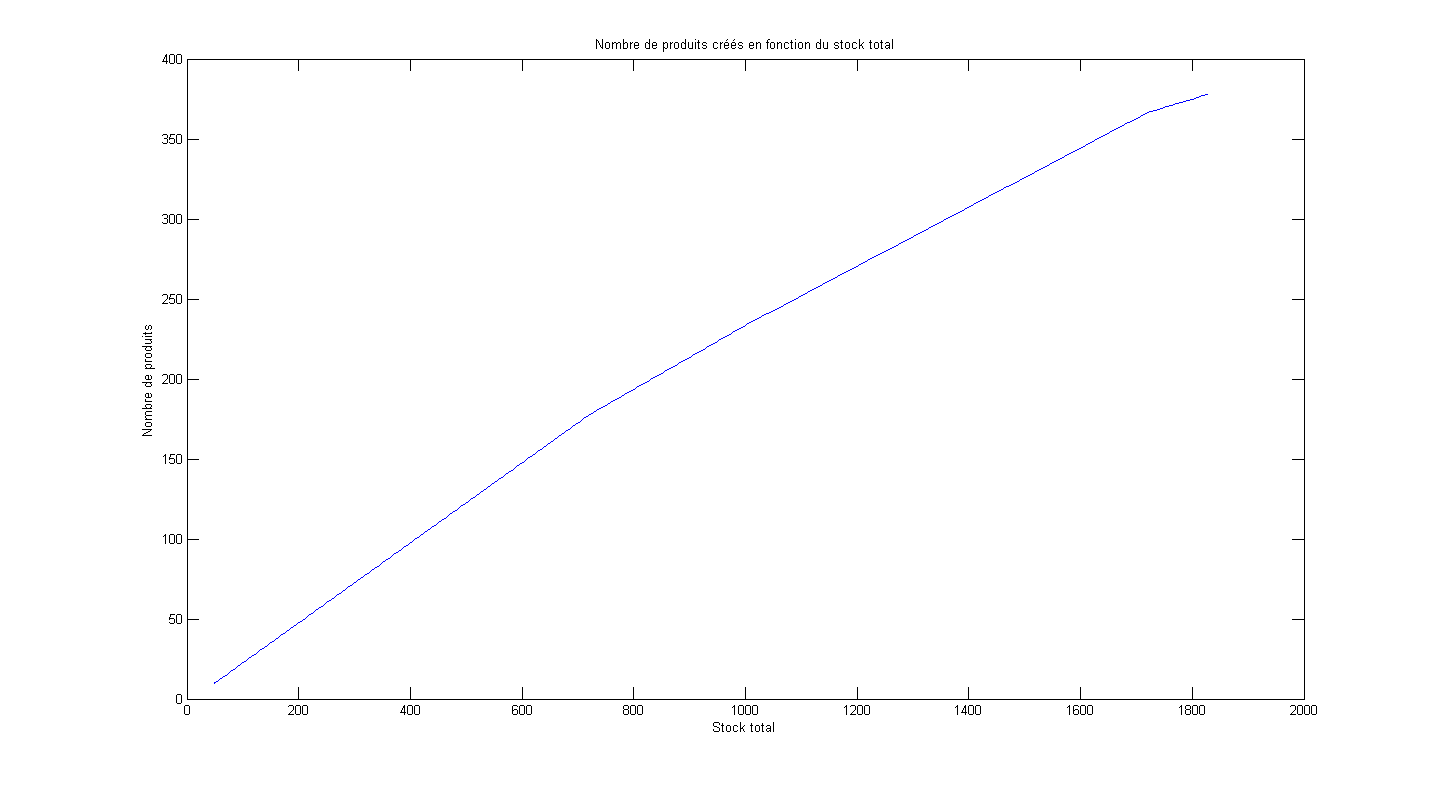
\includegraphics[width=16cm]{figures/nbProduitsFctStockTotal.png}
\end{figure}

\begin{figure}[H]
\caption{Variation du coefficient de la courbe de la figure \ref{figstock}}
\centering
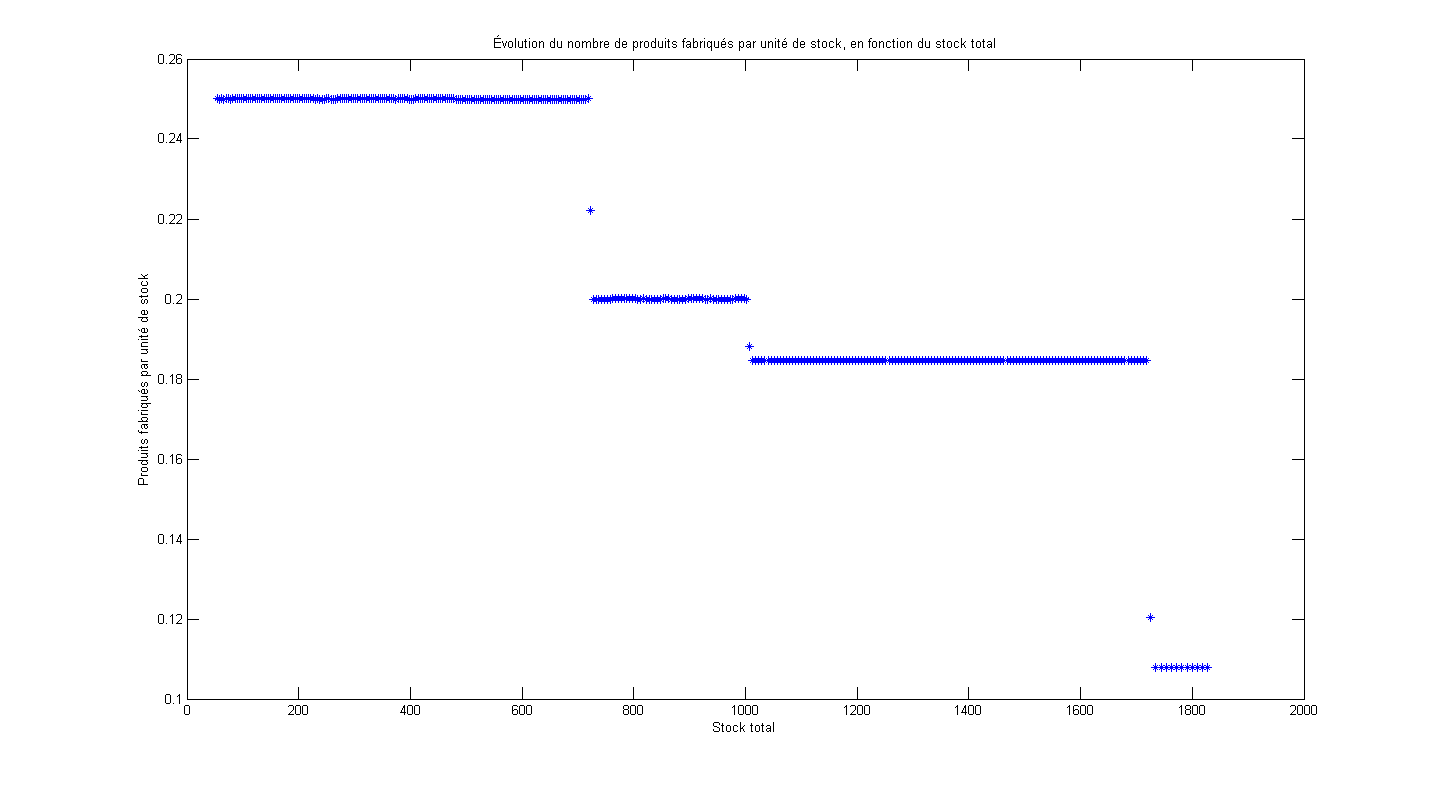
\includegraphics[width=16cm]{figures/nbProduitsFctStockTotal_Coeff.png}
\end{figure}

\begin{figure}[H]
\caption{Bénéfice réalisé en fonction du stock total \label{figben}}
\centering
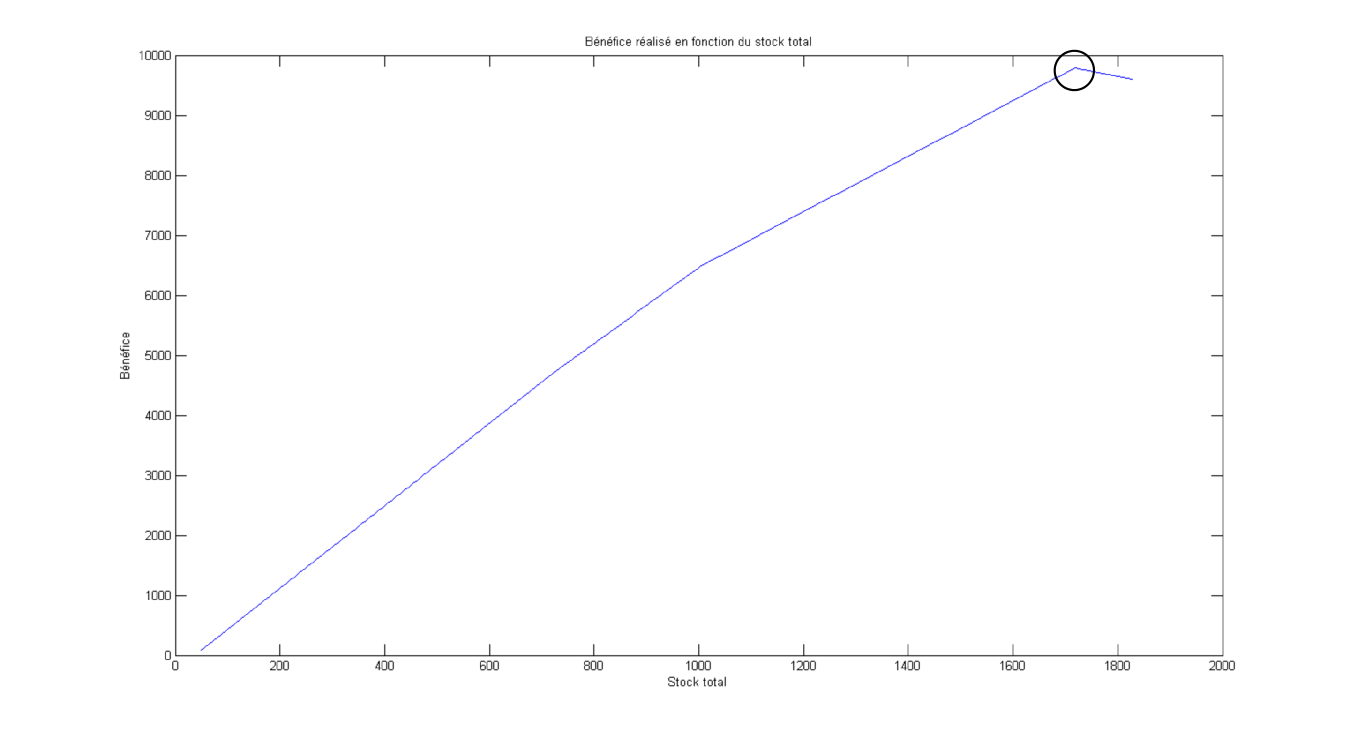
\includegraphics[width=16cm]{figures/BenefFctStockTotal.png}
\end{figure}

\begin{figure}[H]
\caption{Variation du coefficient de la courbe de la figure \ref{figben}}
\centering
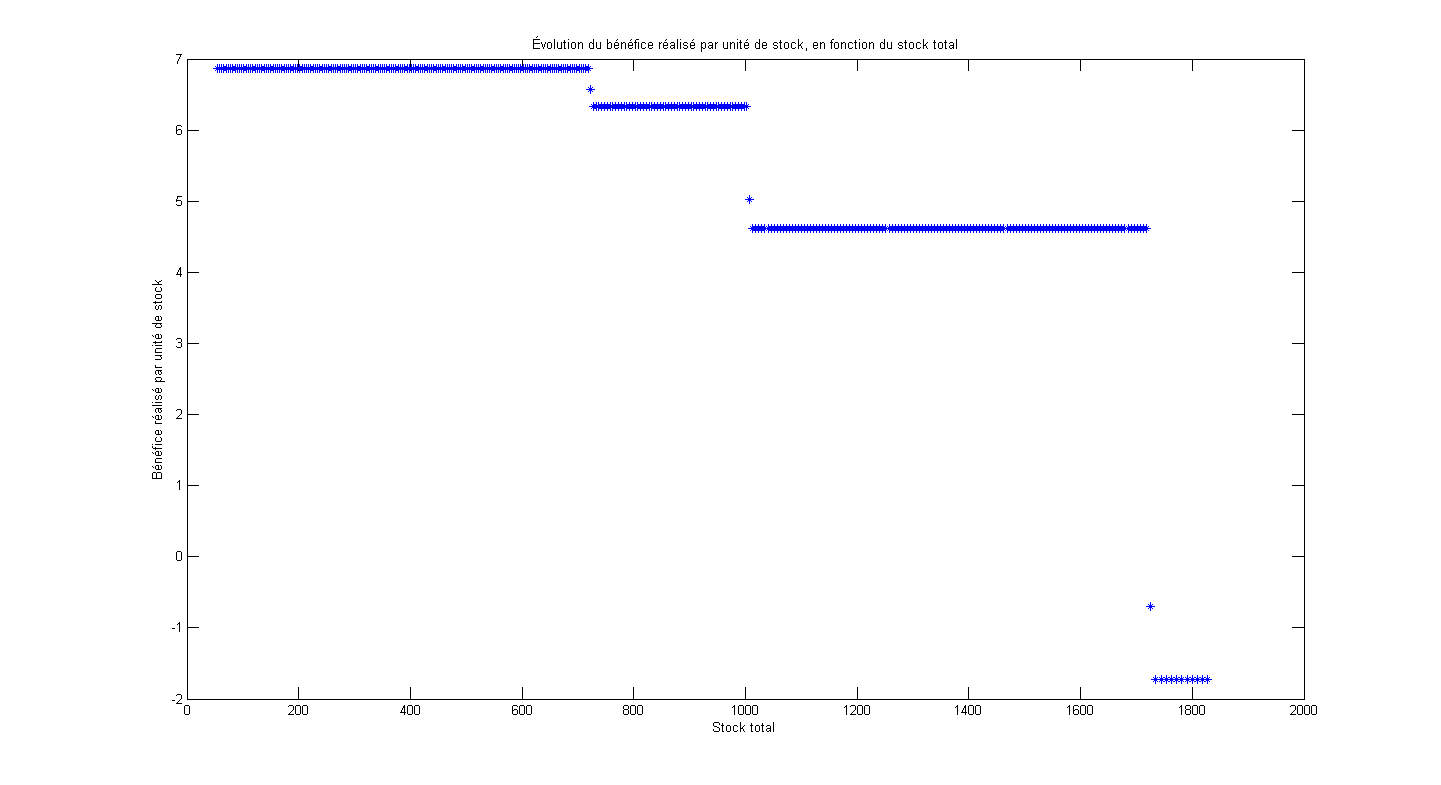
\includegraphics[width=16cm]{figures/BenefFctStockTotal_Coeff.png}
\end{figure}


Les figures montre que pour une production réaliste de produits fabriqués ($> 200$), on peut voir que la rentabilité par produit chute à partir de 1003 unités de stocks, soit une production de 243 produits dont Matlab nous donne la répartition.

\begin{center}
\begin{tabular}{cccccc}
\hline 
$q_A$ & $q_B$ & $q_C$ & $q_D$ & $q_E$ & $q_F$ \\ 
\hline 
5,00 & 5,00 & 0,00 & 0,00 & 56,5 & 167,5 \\ 
\hline 
\end{tabular} 
\end{center}

Un autre point peut également être considéré pour évaluer une répartition optimale des stocks. Il s'agit du dernier point où on constate une variation brutale du coefficient directeur des courbes (qui correspond à 1717 unités de stocks, 366 produits, ou encore un bénéfice de 9786 €). A cet endroit, on obtient la répartition du stock suivante :

\begin{center}
\begin{tabular}{cccccc}
\hline 
$q_A$ & $q_B$ & $q_C$ & $q_D$ & $q_E$ & $q_F$ \\ 
\hline 
5.00 & 53,23 & 0,00 & 0,00 & 172,50 & 119,27 \\ 
\hline 
\end{tabular} 
\end{center}

Le deuxième choix a l'inconvénient d'être moins rentable niveau bénéfice/stockage mais présente l'avantage d'être mieux en accord avec le nombre de produits à produire vis-à-vis des autres responsables.

%%%%%%%%%%%%%%%%%%%%%%%%%%%%%%%%%%%%%%%%%%%%%%%%%%%%%%%% RESP COMMERCIAL %%%%%%%%%%%%%%%%%%%%%%%%%%%%%%%%%%%%%%%%%%%%%%%%%%%%%%%%
\section{Responsable commercial}
\bf{Problème soumis :}

Le responsable commercial souhaite pour sa part équilibrer la quantité de produite des produits A et E.\\

\bf{Solution proposée :}

Suite à notre étude du problème, c'est à dire la maximisation des bénéfices en équilibrant la production des produits A et E, plusieurs constats peuvent être faits :\\

\bf{Contraintes supplémentaires :}

La contrainte supplémentaire qui est ajouté est donc de faire en sorte que $q_A = q_E$. 

On ajoute donc la contrainte suivante pour minimiser l'écart en $q_A$ et $q_E$ : \[ \abs{q_A - q_E} \leq \epsilon \] 

Pour un écart nul entre les quantités de A et E produites on a les quantités hebdomadaires suivantes suivants :
\begin{center}
\begin{tabular}{cccccc}
\hline
$q_A$ & $q_B$ & $q_C$ & $q_D$ & $q_E$ & $q_F$ \\
\hline
119.08 & 6.91 & 42.58 & 0.00 & 119.08 & 87.24 \\
\hline
\end{tabular}
\end{center}
Tout d'abord le produit D ne semble pas rentable car l'étude conclue qu'il serait optimal de ne plus le produire du tout.
On remarque également que l’évolution de e tend à favoriser la production du produit E plutôt que le produit A.

%%%%%%%%%%%%%%%%%%%%%%%%%%%%%%%%%%%%%%%%%%%%%%%%%%%%%%%% RESP DU PERSONNEL %%%%%%%%%%%%%%%%%%%%%%%%%%%%%%%%%%%%%%%%%%%%%%%%%%%%%%%%
\section{Responsable du personnel}
\bf{Problème soumis :}

Le responsable du personnel souhaite utiliser le moins possible la machine 4.\\

\bf{Solution proposée :}

La première solution qui nous vient à l’esprit serait de minimiser la fonction suivante :\[f(Q) = 2q_A + 10q_B + 5q_C + 4q_D + 13q_E + 7q_F\]

Cependant, les résultats que l’on obtient en ne prenant en compte que cette équation ne sont pas satisfaisant, car on se retrouverait à ne produire que 5 unités de A et B et 0 des autres. Ce résultat est mathématiquement juste au vu des contraintes que nous avions précisé, mais ne suffit pas pour garder une rentabilité à l’entreprise. Pour trouver une solution plus juste, nous allons prendre en compte une certaine quantité d’unités minimales à produire. \\

Nous reprenons donc les résultats obtenus par le responsable d’atelier, et en faisant varier les différentes quantités de produits fabriqués selon sa méthode de calcul, nous avons établi un graphique permettant d’évaluer le temps d’utilisation de la machine 4.\\

\begin{figure}[H]
\caption{Temps d'utilisation de la machine 4 en fonction du nombre de produits fabriqués}
\centering
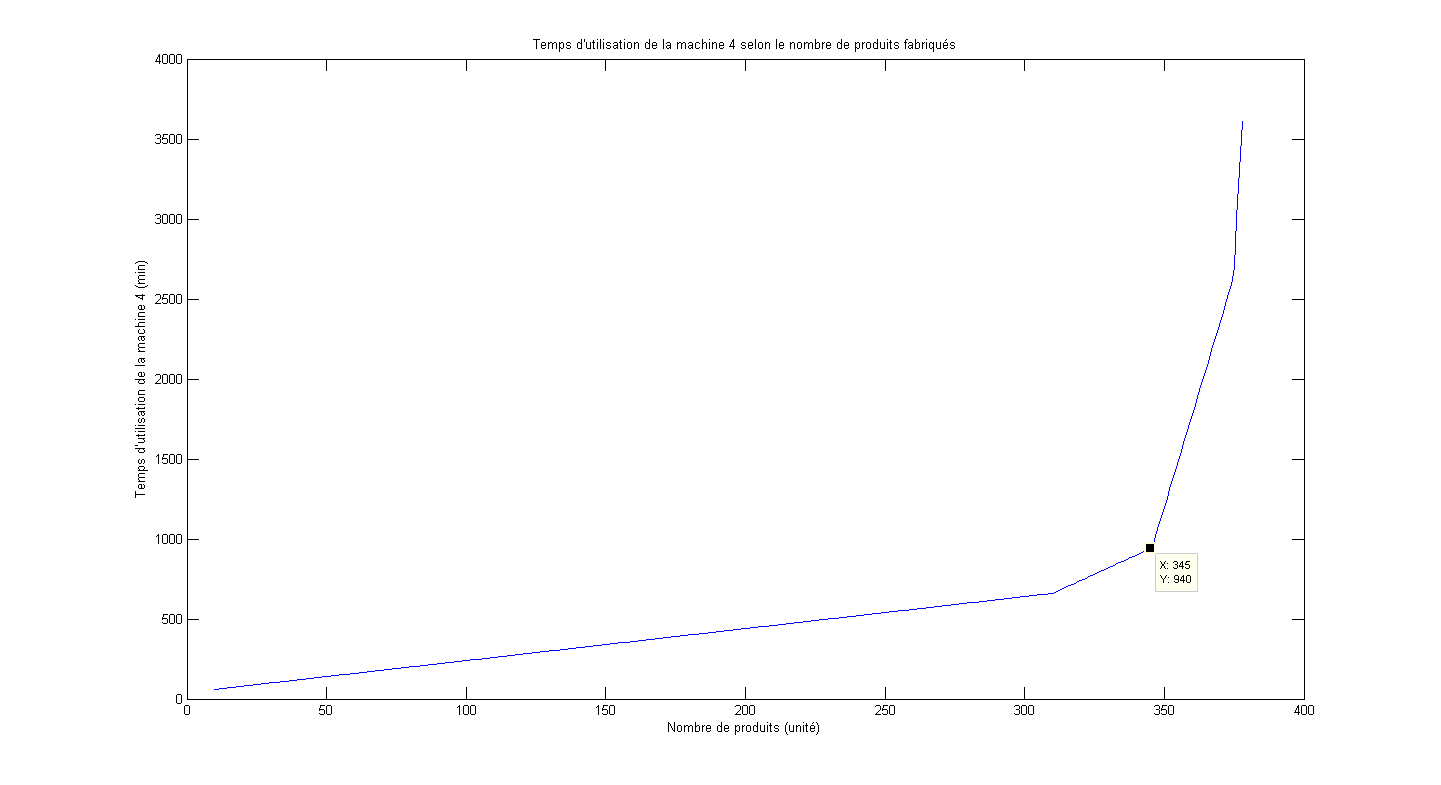
\includegraphics[width=16cm]{figures/graphe-personnel.png}
\end{figure}

On constate très clairement que la pente de la courbe augmente fortement à partir de 345 unités fabriquée, ce qui correspond à 940 min de travail pour la machine 4. Au delà de ce seuil, on utilise beaucoup plus la machine 4.\\

345 étant la limite à jusqu'à laquelle on peut produire le plus d’unités en utilisant le moins la machine 4, on choisira donc arbitrairement un minimum de 345 unités à fabriquer.

\begin{center}
\begin{tabular}{cccccc}
\hline
$q_A$ & $q_B$ & $q_C$ & $q_D$ & $q_E$ & $q_F$ \\
\hline
270.00 & 5.00 & 70.00 & 0.00 & 0.00 & 0.00 \\
\hline
\end{tabular}
\end{center}


\section{Bilan}

Voici le tableau récapitulatif pour les différents acteurs de l'entreprise :

\begin{center}
\begin{tabular}{l|cccccc|cc}
\hline
Responsables & $q_A$ & $q_B$ & $q_C$ & $q_D$ & $q_E$ & $q_F$ & $\sum q_i \quad$ & Point de Mire \\
\hline
Comptable & 5,00 & 18,00 & 0,00 & 0,00 & 240,00 & 93,67 & 356,67 & $10 \:048\,$€\\
Responsable d'atelier & 5,00 & 54.64 & 38,85 & 0,00 & 181,71 & 98,43 & 378,63 & 378,63 produits\\
Responsable des stocks & 5,00 & 5,00 & 0,00 & 0,00 & 56,5 & 167,5 & 234,00 & $1\:003\,$ unités de stocks\\
Responsable commercial & 119.08 & 6.91 & 42.58 & 0.00 & 119.08 & 87.24 & 374,89 & $\frac{q_A}{q_E}=1$\\
Responsable personnel & 270.00 & 5.00 & 70.00 & 0.00 & 0.00 & 0.00 & 345,00 & $940\,$ min \\

\hline
\end{tabular}
\end{center}
%%%%%%%%%%%%%%%%%%%%%%%%%%%%%%%%%%%%%%%%%%%%%%%%%%%%%%%%%%%%%%%%%%%%%%%%%%%%%%%%%%%%%%%%%%%%%%%%%%%%%%%%%%%%%%%%%%%%%%%%%%%%%%%%
%%%%%%%%%%%%%%%%%%%%%%%%%%%%%%%%%%%%%%%%%%%%%%%%%%%%%%%% RESP DES STOCK %%%%%%%%%%%%%%%%%%%%%%%%%%%%%%%%%%%%%%%%%%%%%%%%%%%%%%%%
%%%%%%%%%%%%%%%%%%%%%%%%%%%%%%%%%%%%%%%%%%%%%%%%%%%%%%%%%%%%%%%%%%%%%%%%%%%%%%%%%%%%%%%%%%%%%%%%%%%%%%%%%%%%%%%%%%%%%%%%%%%%%%%%
\part{\'Etude du problème soumis par le Responsable de l'entreprise}



\part{Analyse Multicritère}

\section{Introduction et choix de la méthode de résolution}
Le but est de choisir la meilleure solution parmi toutes celles proposées. Pour cela, la méthode \textbf{Electre 1} nous a paru être la plus adaptée.

La matrice de jugement a été reproduite ci-dessous. Celle-ci représente l'importance des critères $g_1$, $g_2$, $g_3$ et $g_4$ sur une échelle de 0 à 10. Ces critères sont : 

\begin{multicols}{2}

\begin{itemize}
\item $g_1$ : le bénéfice
\item $g_2$ : la gestion du stock
\item $g_3$ : l'équilibre commercial
\item $g_4$ : l'utilisation de la machine 4
\end{itemize}


\begin{table}[H]
\begin{center}
\begin{tabular}{c|cccc}
 & $g_1$ & $g_2$ & $g_3$ & $g_4$ \\ 
\hline 
a & 6 & 5 & 5 & 5 \\ 
b & 5 & 2 & 6 & 7 \\ 
c & 3 & 4 & 7 & 3 \\ 
d & 3 & 7 & 5 & 4 \\ 
e & 5 & 4 & 3 & 9 \\ 
f & 2 & 5 & 7 & 3 \\ 
g & 5 & 4 & 2 & 9 \\ 
h & 3 & 5 & 7 & 4 \\ 
\end{tabular}
\caption{Matrice de jugement} 
\end{center}
\end{table}

\end{multicols}


\section{Explication de la démarche}

\subsection{Elimination des solutions dominées}

Nous avons commencé par éliminer les solutions dominées, c’est-à-dire les solutions pour lesquelles il existe une meilleure autre solution pour tous les critères.\\

On constate alors que :

\begin{equation*}
  \left.
    \begin{aligned}
	e & \rightarrow g \\
 h & \rightarrow f \\
 h & \rightarrow c 
    \end{aligned}
  \right. \quad \quad \rightarrow \text{ : “domine”}
\end{equation*}

Chaque critère est pondéré selon les pondérations choisies lors de la programmation multicritère (partie précédente). 
Nous retenons donc un poids de :\\

 \begin{itemize}
\item 4 pout le bénéfice,
\item 1 pour la gestion du stock,
\item 2 pour l’équilibre de la production A/E
\item 1 pour la réduction du temps de la machine 4.\\
\end{itemize}


\begin{table}[H]
\begin{center}
\begin{tabular}{c|cccc}
 & $g_1$ (4) & $g_2$ (1) & $g_3$ (2) & $g_4$ (1) \\ 
\hline 
a & 6 & 5 & 5 & 5 \\ 
b & 5 & 2 & 6 & 7 \\ 
d & 3 & 7 & 5 & 4 \\ 
e & 5 & 4 & 3 & 9 \\ 
h & 3 & 5 & 7 & 4 \\ 
\end{tabular} 
\caption{Nouvelle matrice de jugement\\ 
les poids sont indiqués entre parenthèses} 
\end{center}
\end{table}


Ensuite, à partir de notre nouvelle table de jugement (qui ne contient alors que les solutions non-dominées), nous avons écrit les matrices de concordance et de discordance. La matrice de concordance montre la similarité entre deux solutions, tandis que la matrice de discordance montre plutôt les écarts.\\

\subsection{Matrice de concordance}

\begin{equation*}
C(A_i, A_j) = \frac{\mathlarger{\mathlarger{\sum}}\limits_{\mathsmaller{k \in P^+ \cup P^=}} p_k}{\mathlarger{\mathlarger{\sum}}\limits_{\mathsmaller{I \in P}} p_I}
\end{equation*} 

On calcule la somme des poids des critères pour lesquels la solution $i$ est meilleure que la $j$, puis on la divise par la somme totale des poids de tous les critères.\\

\begin{table}[H]
\begin{center}
\begin{tabular}{c|ccccc}
 & a & b & d & e & h \\ 
\hline 
a & 0 & 0.50 & 0.75 & 0.75 & 0.75 \\ 
b & 0.50 & 0 &	0.75 &	 0.50 & 0.50 \\ 
d & 0.50 & 0.25 & 0 & 0.50 & 0.75 \\ 
e & 0.25 & 0.75 & 0.50 & 0 & 0.50 \\ 
h & 0.50 & 0.50 & 0.75 & 0.50 & 0\\ 
\end{tabular} 
\caption{Matrice de concordance} 
\end{center}
\end{table}



\subsection{Matrice de discordance} 

\begin{equation*}
D(A_i, A_j) = \frac{\mathlarger{\mathlarger{\text{Max}}}_{\mathsmaller{k \in P^- }} (e_{jk} - e_{ik})}{\text{echmax}}
\end{equation*} 

On compare la solution $i$ et la $j$. On récupère la plus grande valeur de la différence entre la note de $j$ et la note de $i$, tous critères compris. Puis on divise cette valeur par l’échelle la plus grande.\\


\begin{table}[H]
\begin{center}
\begin{tabular}{c|ccccc}
 & a & b & d & e & h \\ 
\hline 
a & 0 & 0.20	 & 0.20 & 0.40 & 0.20 \\ 
b & 0.30 & 0	& 0.50 & 0.20 &	0.30 \\ 
d & 0.30 & 0.30 & 0 & 0.50 &	0.20 \\ 
e & 0.20 & 0.30 & 0.30 & 0 & 0.40 \\ 
h & 0.30 & 0.30 & 0.20 &	0.50 & 0\\ 
\end{tabular} 
\caption{Matrice de discordance} 
\end{center}
\end{table}

\subsection{seuillage des résultats}

Finalement, nous choisissons tout d’abord un seuil de concordance, qui correspond à la similarité que l’on tolère entre nos solutions. Ensuite, nous prenons un seuil de discordance, qui correspond à l’écart que l’on tolère entre nos solutions. Ils sont tous les deux compris entre 0 et 1, comme toutes les valeurs de nos matrices de concordance et discordance.\\

\begin{itemize}
\item \bf{Seuil de concordance :} 0,7
\item \bf{Seuil de discordance :} 0,3 puis 0,5 (le seuil à 0,3 ne donnant pas un graphe concluant, nous avons légèrement augmenté notre tolérance au niveau de la discordance)
\end{itemize}

\section{Résultats}

À partir de ces seuils, nous avons pu définir quelle solution dominait les autres de la façon suivante : \\
Soit une solution A. On la compare avec une autre solution B. Si la discordance de A par rapport à B est inférieure au seuil de discordance et que la concordance de A par rapport à B est supérieure au seuil de concordance, alors la solution A domine la B.\\

Voici les résultats obtenus avec un seuil de concordance de 0.7 et un seuil de discordance de 0.5 : 
\begin{multicols}{2}

\begin{table}[H]
\begin{center}
\begin{tabular}{c|ccccc}
 & a & b & d & e & h \\ 
\hline 
a & 0 & 0 & 1 & 1 & 1 \\ 
b & 0 & 0 & 1 & 1 & 0 \\ 
d & 0 & 0 & 0 & 0 & 1 \\ 
e & 0 & 1 & 0 & 0 & 0 \\ 
h & 0 & 0 & 1 & 0 & 0\\ 
\end{tabular} 
\caption{Matrice de surclassement} 
\end{center}
\end{table}
\begin{figure}[H]
\centering
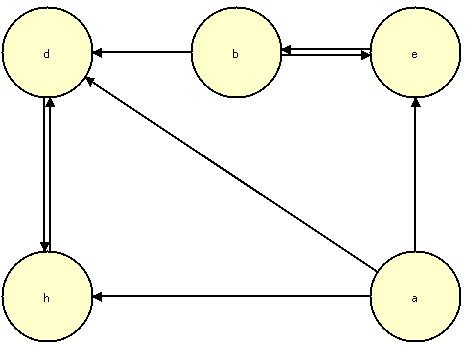
\includegraphics[width=5cm]{figures/GraphDeSurClassement.png}
\caption{Graphe de surclassement}
\end{figure}
\end{multicols}

Avec le seuil de discordance à 0,5, on peut conclure que \textbf{la solution A est la meilleure car elle surclasse les autres et elle n'est pas surclassée} (cf. graphe de surclassement).\\

Cependant, avec le seuil de discordance à 0,3 (donc un peu plus sévère), la solution A semble être à peu près équivalente à la E. En effet, la solution E est assez disparate (certains critères remportent une excellente note, tandis que d’autres critères ont une note très basse), alors que la A est beaucoup plus homogène. Le choix de la meilleure solution entre ces deux-là se fait donc en fonction de notre tolérance à la compensation des notes entre elles.


\begin{appendices} 
\lstlistoflistings

\lstinputlisting[caption=Comptable]{scripts/Comptable.m}
\lstinputlisting[caption=Responsable Atelier]{scripts/ResponsableAtelier.m}
\lstinputlisting[caption=Responsable Commercial]{scripts/ResponsableCommercial.m}
\lstinputlisting[caption=Responsable Stocks]{scripts/ResponsableStock.m}
\lstinputlisting[caption=Responsable Personel]{scripts/ResponsablePersonnel.m}
\newpage
\lstinputlisting[caption=Programation Linéaire Multicritère]{scripts/partie2.m}
\newpage
\lstinputlisting[caption=Analyse Multicritère]{scripts/partie3.m}

\end{appendices} 

%%% End document
\end{document}
